%!TEX program = xelatex
% \documentclass[dvips,11pt]{beamer}
    \documentclass{beamer}
        \usepackage{xeCJK,subfigure}
        % \setCJKmainfont{Adobe Song Std}
        % \setCJKmainfont{楷体}
        \setbeamertemplate{footline}[frame number] %添加页码
        % \usetheme{Warsaw}
        \usecolortheme{rose}
        % \title{你好!beamer}
        \date{2017 11}
    \begin{document}
    
    % \begin{frame}
    %     \titlepage
    % \end{frame}
    
    \begin{frame}
        \frametitle{目录}
        \tableofcontents
        % \tableofcontents[pausesections]   
    \end{frame}
    
    % \section{性能比较}
    % \begin{frame}
    %     \frametitle{准确率与耗时}
    %     \begin{itemize}
    %         \item R-CNN \\
    %         在20类的 PASCAL VOC 2010上mAP达到53.7\%,而以往的DPM在这个数据集上是33.4\%,在200类数据集ILSVRC 2013上的目标检测数据集上,mAP是31.4\%
    %         耗时:在GPU上一张图像生成proposal box和提取特征耗时13s,cpu上耗时53s
    %     \end{itemize}
    % \end{frame}
    
    % rcnn
    \section{R-CNN 2013}
    
    \begin{frame}
        \frametitle{数据流程图}
        \framesubtitle{2013 Rich feature hierarchies for accurate object detection and semantic segmentation}
        \begin{figure}
            \centering
            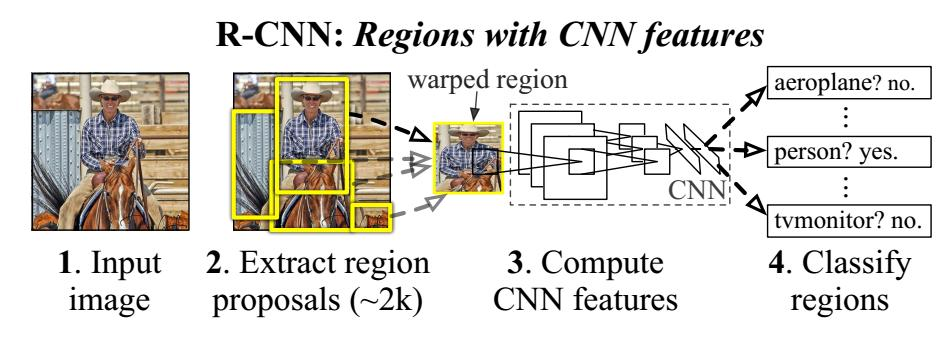
\includegraphics[height=4cm]{../graphic/rcnnflow.jpg}
        \end{figure}
        输入:图像及selective search算法提出的2000个proposal box。  \\
        输出:proposal box包含的目标类别,及修正后的位置坐标。  \\
    \end{frame}
    
    \begin{frame}
        \frametitle{proposal box的形状变换}
        % \framesubtitle{proposal box的变换}
        \begin{figure}
            \centering
            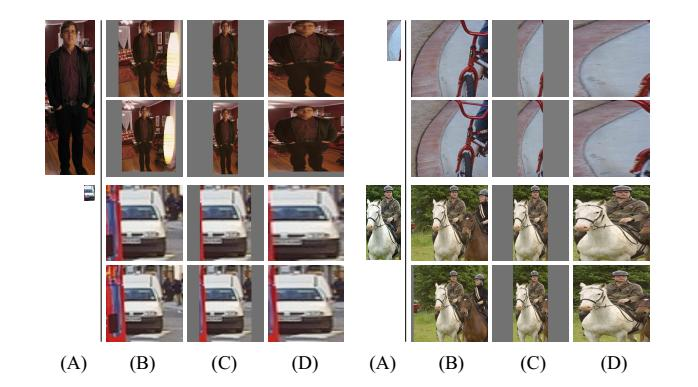
\includegraphics[height=5cm]{../graphic/rcnnwarp.jpg}
        \end{figure}
        \scriptsize{A是原图的proposal box,B是proposal box的最小外接正方形,短边使用原图填充,然后放大到$227\times 227$,C与B的相同,只是填充短边时使用图像均值,D是直接 warp,即直接进行放大。每列图像,上一行是直接对proposal box处理,即 context padding = 0,下一行的 context padding = 16。实验表明使用D方法中的 warp with context padding = 16时,效果最好,提高3-5 mAP\%}
    \end{frame}
    
    \begin{frame}
        \frametitle{特征提取网络}
        \begin{figure}
            \centering
            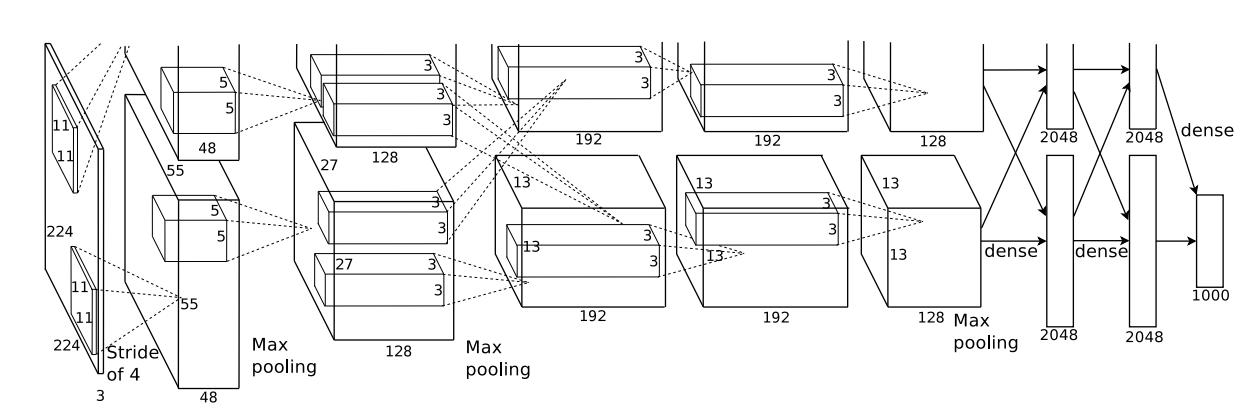
\includegraphics[height=3.7cm]{../graphic/alexnet.jpg}
        \end{figure}
        采用了和Alexnet一样的结构,5层卷积,3层全连接的分类网路。在做特征提取时,只计算到第二层全连接输出4096维特征向量。
    \end{frame}
    
    \begin{frame}
        \frametitle{proposal box的分类}
        这里使用category-specific linear SVM对上一步中proposal box中提取的$4096$维特征向量进行分类。 \\
        \vspace{10pt}
        测试时,一张图像提出$2000$个proposal box,对应的特征向量写成一个矩阵就是$2000\times 4096$维, 乘以 SVM系数矩阵$4096\times N$ (N指目标类别数目)得到每一个proposal box的分数。%之后使用单独为每一类的输出做非极大值抑制,就是去掉那些与有更高分数的proposal box的IOU超过一个阈值的框。
    \end{frame}
    
    \begin{frame}
        \frametitle{class-specific bounding box regressor}
        proposal box的参数表示: $P^i=(P_x^i,p_y^i,p_w^i,p_h^i)$ \\
        ground truth box的参数表示: $G=(G_x^i,G_y^i,G_w^i,G_h^i)$ \\
        回归的目标: \\
        $$\begin{aligned} 
            t_x &= (G_x-P_x)/P_w \\
            t_y &= (G_y-P_y)/P_h \\
            t_w &= \log(G_w/P_w)=\log(G_w)-\log(P_w) \\
            t_h &= \log(G_h/P_h)=\log(G_h)-\log(P_h)
        \end{aligned}$$
        \vspace{6pt}
        回归使用的是线性模型,损失函数是均方误差加上$L_2$正则项: 
        $$loss=\sum_i^N (t_{\star}^i-\hat w_{\star}^T \phi_5(P^i))^2+\lambda\|\hat w_{\star}\|^2$$
        \scriptsize{其中,$\phi_5(P^i)$表示CNN的pool 5层在proposal box内提取的特征,$w_{\star}$表示回归要学习的参数。}
    \end{frame}
    
    \begin{frame}
        \frametitle{log space error的作用}
        \begin{figure}
            \centering
            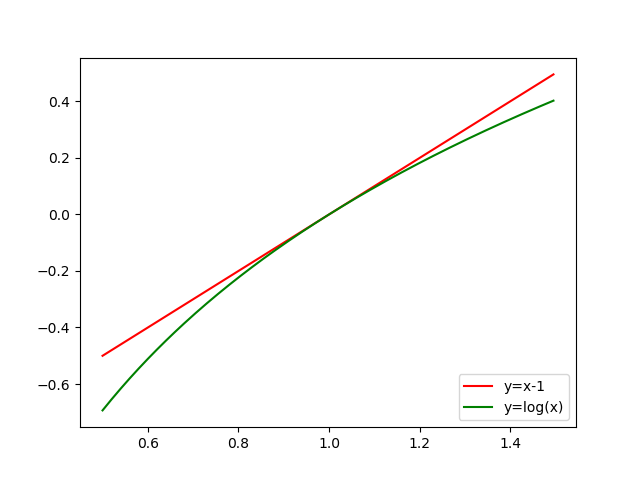
\includegraphics[height=6.5cm]{../graphic/log.png}
        \end{figure}
        \scriptsize{对不同大小的box预测,相比于大box的长、宽预测偏一点,小box预测长、宽的偏差是更不能忍受的,而sum-squared error loss中对同样的偏差loss是一样的,所以要采取一种方式来增大小box的预测偏差损失的权重}
    \end{frame}

    \begin{frame}
        \frametitle{IOU}
        Intersection Over Union:两个框重叠度的计算 \\
        \begin{figure}
            \centering
            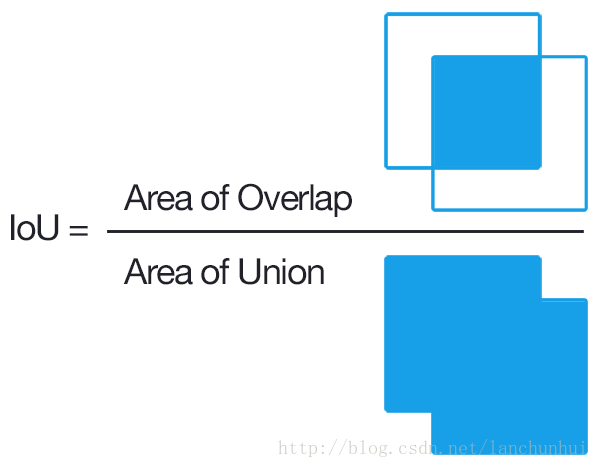
\includegraphics[height=4cm]{../graphic/iou.png}
        \end{figure}
    \end{frame}
    
    \begin{frame}
        \frametitle{训练}
        \begin{itemize}
            \item CNN的训练 \\
            先在ILSVRC2012图像分类数据集上进行预训练,之后在目标检测数据集VOC与ILSVRC203上进行微调,微调时把proposal box中所有与ground-truth box的IOU大于0.5的框看做正样本,其余的proposal box都是负样本。训练时,batch-size为128,其中32个为正样本,96个背景样本。        
            \item SVM的训练样本 \\
            正样本只有ground-truth box提出的特征,负样本是propoal box中与ground-truth box的IOU小于0.3的。
            \item bounding-box regressor的训练样本   \\
            对于每一个proposal box,计算它与所有的ground-truth box的IOU,然后选出IOU最大的那一个,如果此IOU值大于$0.6$,那么这个proposal box就配对成功,看做一个训练样本,配对不成功的proposal box被舍弃。
        \end{itemize}
    \end{frame}
    
    % fast rcnn
    \section{Fast R-CNN 2015}
    
    \begin{frame}
        \frametitle{数据流程图}
        \framesubtitle{2015 Fast R-CNN}
        \begin{figure}
            \centering
            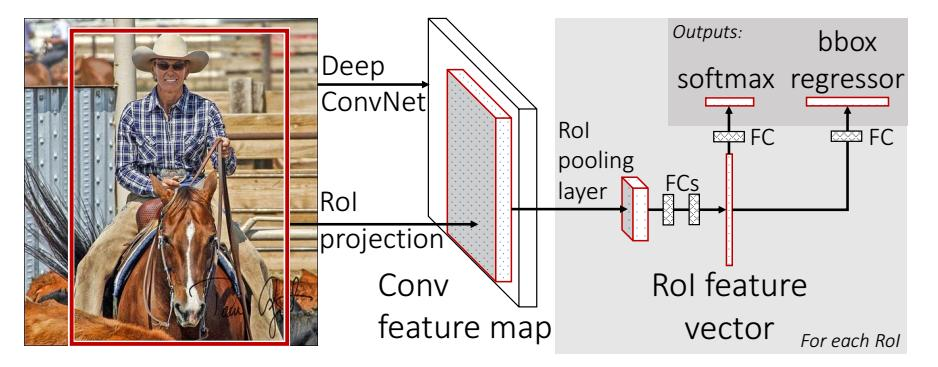
\includegraphics[height=4.3cm]{../graphic/fastrcnnflow.jpg}
        \end{figure}
        输入:图像及selective search算法提出的2000个proposal box。  \\
        输出:proposal box包含的目标类别,及修正后的位置坐标。  \\
    \end{frame}
    
    % \begin{frame}
    %     \frametitle{ROI pooling}
    %     ROI:region of interest,就是特征图上的一个矩形,对应到原图的proposal box, \\
    %     \begin{figure}
    %         \centering
    %         \includegraphics[width=0.35\textwidth]{../graphic/roipooling0.jpg}%
    %         \includegraphics[width=0.35\textwidth]{../graphic/roipooling1.jpg}%
    %         \includegraphics[width=0.35\textwidth]{../graphic/roipooling2.jpg}
    %     \end{figure}
    %     卷积网络输出为$8\times 8$的特征图,这里的一个左上角坐标为$(0,3)$,右下角坐标为$(6,7)$,长宽分别为$7,5$的roi一个Roi对应$2\times 2$的固定长度的特征向量输出。
    % \end{frame}
    
    % \begin{frame}
    %     \frametitle{ROI pooling}
    %     \begin{figure}
    %         \centering
    %         \includegraphics[width=0.5\textwidth]{../graphic/roipooling3.jpg}%
    %         \includegraphics[width=0.5\textwidth]{../graphic/roipooling4.jpg}%
    %     \end{figure}
    %     Roi pooling使不同大小,不同长宽比的proposal box都能提取到固定长度的特征向量。
    % \end{frame}
    \begin{frame}
        \frametitle{ROI pooling}
        \begin{figure}
            \centering
            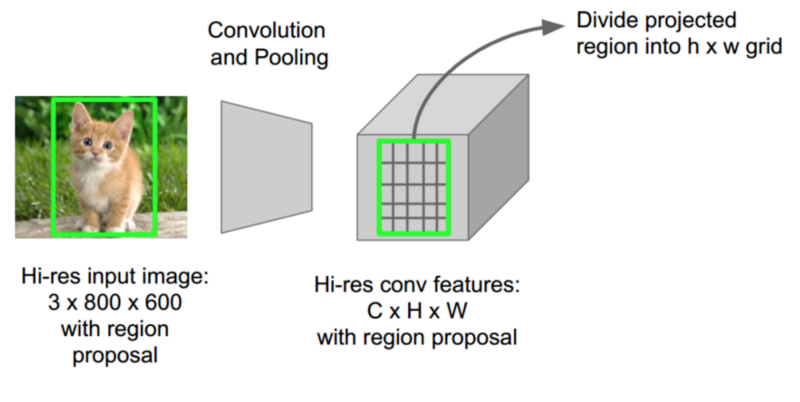
\includegraphics[width=1.0\textwidth]{../graphic/roipooling6.png}
        \end{figure}
        Roi pooling使不同大小,不同长宽比的proposal box都能提取到固定长度的特征向量。
    \end{frame}
    
    
    \begin{frame}
        \frametitle{Multi-task loss}
        分类器与坐标回归的损失函数:
        $$L(p,u,t^u,v)=L_{cls}(p,u) + \lambda [u\geqslant 1]L_{loc}(t^u,v)$$
        其中,p为预测的分类概率,u真实分类的label,$t^u$为预测的坐标偏差,因为坐标回归针对每一类都有一个回归器,所以它是$u$的函数,v为真实的坐标偏差label,$[u\geqslant 1]$艾佛森括号,表示$u\geqslant 1$时,输出为1,否则为0。
    \end{frame}
    
    \begin{frame}
        \frametitle{Multi-task loss}
        分类器与坐标回归的损失函数:
        $$L(p,u,t^u,v)=L_{cls}(p,u) + \lambda [u\geqslant 1]L_{loc}(t^u,v)$$
        分类损失:
        $$L_{cls}=-\log p_u$$
        坐标回归损失:
        $$L_{loc}(t^u,v)=\sum_{i\in \{x,y,w,h\}}smooth_{L1}(t^u_i-v_i)$$
        与R-CNN不同,这里使用了$Smooth_{L1}$损失:
        $$smooth_{L1}(x) = \begin{cases} 
            0.5x^2 &\text{if }|x| < 1 \\
            |x| - 0.5 &\text{otherwise}\end{cases}  \rightarrow \text{求导}
        \begin{cases} x \\ \pm 1 \end{cases}$$
    \end{frame}
    
    % faster rcnn 2015
    \section{Faster R-CNN 2015}

    \begin{frame}
        \frametitle{数据流程图}
        \framesubtitle{2015 faster rcnn: towards real-time object detection with region proposal networks}
        \begin{minipage}[c]{0.6\linewidth}
            \centering
            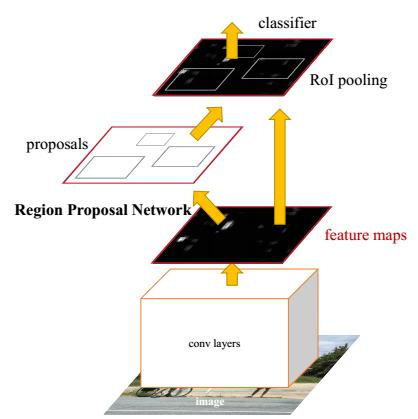
\includegraphics[width=1.0\textwidth]{../graphic/fastercnnflow.jpg}
        \end{minipage}%
        \begin{minipage}[c]{0.45\linewidth}
            Faster R-CNN相当于RPN与Fast R-CNN的结合体,图中左边是RPN,右边是Fast R-CNN。
        \end{minipage}
    \end{frame}
    
    \begin{frame}
        \frametitle{RPN中的多尺度}
        \framesubtitle{Region Proposal Network}
        \begin{figure}
            \centering
            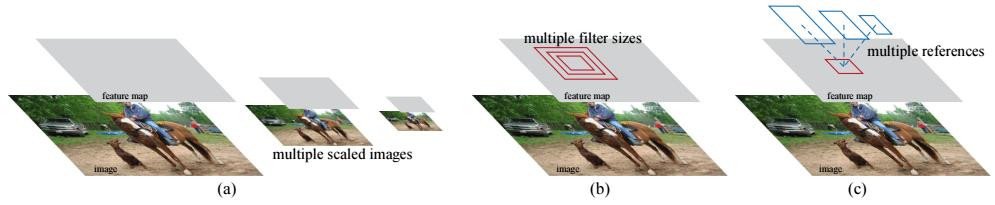
\includegraphics[height=2.3cm]{../graphic/fastermultisize.jpg}
        \end{figure}
        $(a)$通过图像金字塔构造多尺度,$(b)$通过构造滤波器的金字塔构造多尺度,$(c)$使用一个尺度的滤波器,得到一个尺度的特征图,然后在特征图上选不同大小的预设框来构造多尺度。
    \end{frame}
    
    \begin{frame}
        \frametitle{RPN网络的输出}
        \begin{figure}
            \centering
            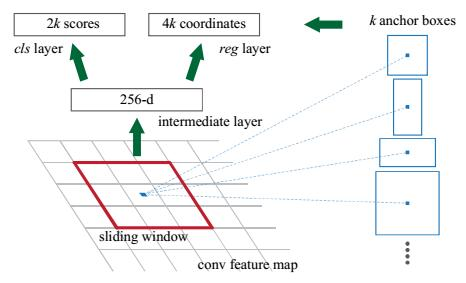
\includegraphics[width=0.8\textwidth]{../graphic/rpnout.jpg}
        \end{figure}
        以$3\times 3$大小的滑动窗口在特征图上滑动,论文中使用的anchor包括$3$种尺寸$128^2,256^2,512^2$及$3$种比例$1:1,1:2,2:1$。
    \end{frame}
    
    \begin{frame}
        \frametitle{RPN网络的损失函数}
        $$L(\{p_i\}, \{t_i\})=\frac{1}{N_{cls}}\sum_i L_{cls}(p_i,p_i^*)+\lambda \frac{1}{N_{reg}}\sum_i p_i^* L_{reg}(t_i,t_i^*)$$ \\
        $p_i$表示预测的一个anchor为目标的概率,\\
        $p_i^*$表示一个anchor的label,为1或0,\\
        $t_i$表示一个anchor上预测的参数化的bounding box,\\
        $t_i^*$表示一个anchor上的ground truth box标签。 
    \end{frame}
    \begin{frame}
        \frametitle{Faster R-CNN的训练}
        1,单独训练RPN;\\
        2,使用步骤中1得到的区域生成方法单独训练Fast R-CNN; \\
        3,使用步骤2得到的网络作为初始网络训练RPN;\\
        4,再次训练Fast R-CNN, 微调参数。\\
    \end{frame}
    
    \begin{frame}
        \frametitle{R-CNN, Fast R-CNN, Faster R-CNN测试时的耗时}
        selective search是一种提出proposal box的方法,在CPU上运行耗时2s每帧
        \begin{table}  
            \centering  
            \begin{tabular}{|l|p{6cm}|}  
                  \hline Model & Time\\  
                  \hline selective search+R-CNN & 2s+1000*ConvTime+1000*FcTime \\
                  \hline selective search+Fast R-CNN & 2s+1*ConvTime+1000*FcTime  \\
                  \hline Faster R-CNN & 1*ConvTime+1000*FcTime \\
                  \hline
            \end{tabular}  
          \end{table}  
    \end{frame}


    \section{Mask R-CNN 2017}
    
    \begin{frame}
        \frametitle{实例分割}
        \framesubtitle{Mask R-CNN 2017}
        \begin{figure}
            % \centering
            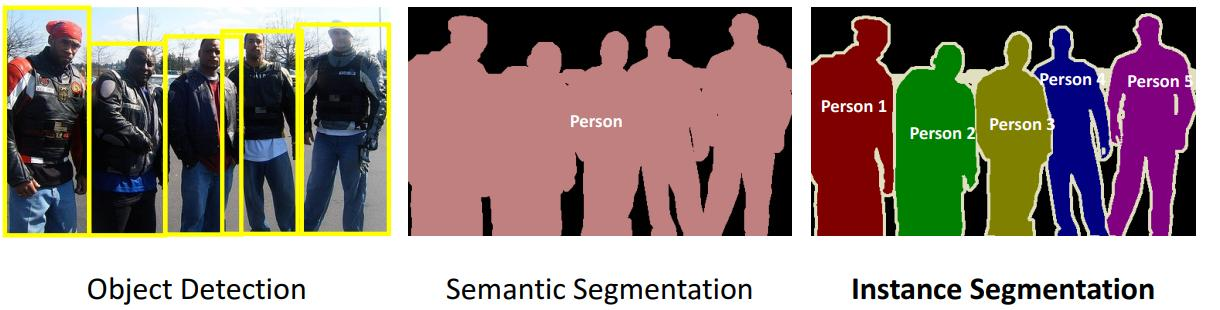
\includegraphics[height=3cm]{../graphic/objseg.jpg}
        \end{figure}
        分别是目标检测,语义分割,实例分割
    \end{frame}

    \begin{frame}
        \frametitle{数据流程图}
        \framesubtitle{Mask R-CNN 2017}
        \begin{figure}
            \centering
            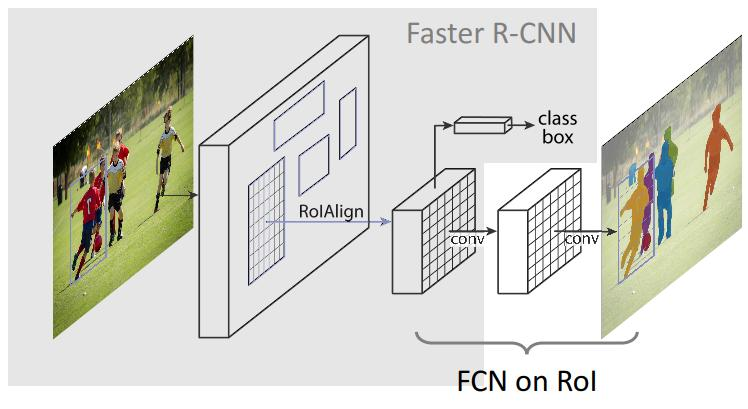
\includegraphics[height=6cm]{../graphic/maskrcnn.jpg}
        \end{figure}
        Mask R-CNN = Faster R-CNN + FCN
    \end{frame}
    
    \begin{frame}
        \frametitle{RoiAlign}
        \begin{figure}
            \centering
            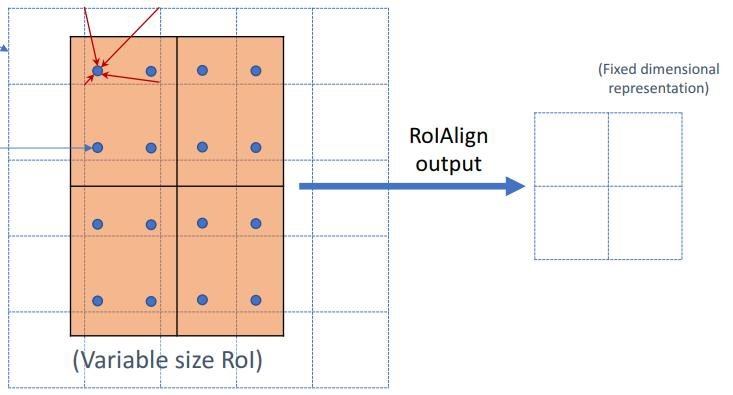
\includegraphics[height=6cm]{../graphic/roialign.jpg}
        \end{figure}
        左侧背景格子表示特征图,棕色格子表示一个Roi被分成$2\times 2$个小格子,蓝色点处的像素值由双线性插值得到。
    \end{frame}

    \begin{frame}
        \frametitle{Roi Pool 中的量化操作}
        \begin{figure}
            \centering
            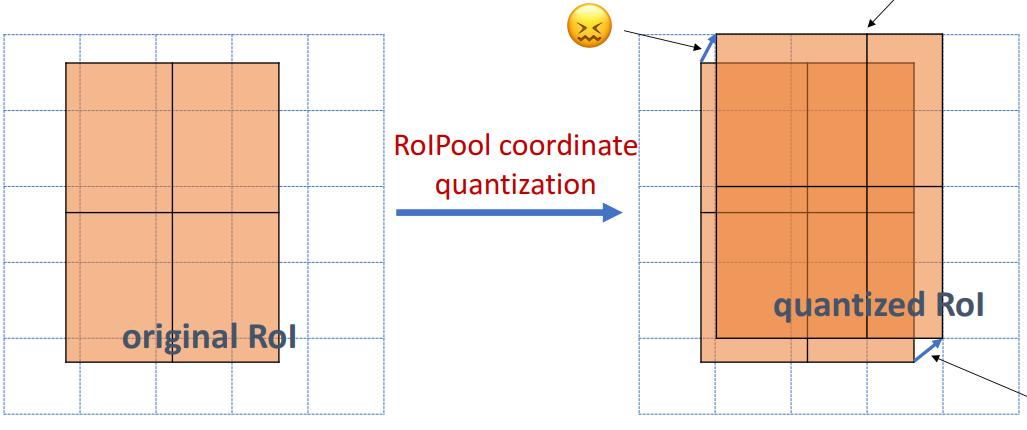
\includegraphics[height=4.5cm]{../graphic/roipoolquanti.jpg}
        \end{figure}
        存在两处量化操作,量化操作导致输出具有平移不变性,会损害实例分割 \\
        \begin{itemize}
            \item 输入图像上的Roi到特征图上的Roi
            \item 特征图上的Roi分成$2\times 2$的小格子
        \end{itemize}
    \end{frame}

    \begin{frame}
        \frametitle{Multi-task Loss}
        \begin{figure}
            \centering
            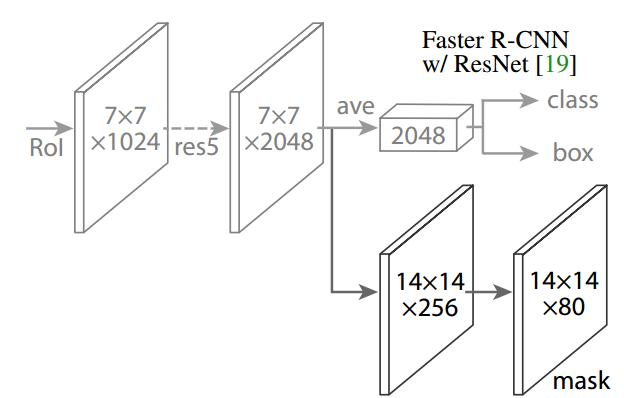
\includegraphics[height=4.5cm]{../graphic/headmask.jpg}
        \end{figure}
        $$L=L_{cls}+L_{box}+L_{mask}$$
        其中前两项与Fast R-CNN中的损失相同,$L_{cls}$是softmax的交叉熵损失,$L_{box}$是Smooth L1损失。\\
        $L_{mask}$是平均二值交叉熵损失。
    \end{frame}

    \begin{frame}
        \frametitle{Mask R-CNN的训练与预测}
        \begin{itemize}
            \item 训练 \\
            $L_{mask}$的训练样本为与ground truth box的IOU大于$0.5$的proposal box。  \\  
            \vspace{20pt}
            \item 预测 \\
            预测时将$14\times 14$的mask直接resize到proposal box的大小,然后以阈值$0.5$对mask做前景、背景的分类。
        \end{itemize}
    \end{frame}

    \end{document}